\documentclass[11pt]{article}
\usepackage[margin=1in]{geometry}
\usepackage{booktabs}
\usepackage{longtable}
\usepackage{amsmath}
\usepackage{graphicx}
\usepackage{hyperref}
\hypersetup{colorlinks=true, linkcolor=blue, urlcolor=blue}

\title{Meeting-Level Information:\\
Deriving It, Validating It Against a Hand-Labelled Gold Set, and What It Shows}
\author{Dan Post}
\date{September 2026}

\begin{document}
\maketitle

\begin{abstract}
\noindent
The item-level dataset needs two things it cannot read off an individual agenda item: the
date the item was heard, and the character of the hearing itself. Both are properties of
the \emph{meeting}. This memo covers how each is derived, how accurate the derivation is
against a hand-labelled gold standard of \textbf{126 documents and 135 meetings}, and what
the resulting data shows.

\medskip\noindent
The gold set was built in \textbf{four rounds}, each scored before the rules had seen it.
\textbf{Meeting dates are correct for 1{,}621 of 1{,}621 items --- 100\% in every round},
and nothing in date assignment has changed since round~1. The meeting-attribute fields
scored \textbf{92.1\%}, \textbf{95.3\%} and \textbf{96.0\%} out-of-sample on rounds 2, 3
and~4; after each round's fixes the figure now stands at \textbf{95.8\%} across the whole
gold set. Round~4 was the first to use \emph{machine-placed} boundaries rather than
hand-marked ones --- the configuration that would run unattended over all 818 meetings ---
and it scored 96.0\% frozen, 98.4\% corrected.

\medskip\noindent
The remaining error is not spread evenly. From 2002 onward the error rate is
\textbf{3.8\%}; for 1999--2001 it is \textbf{11.1\%}, and \textbf{5.7\%} once the
\texttt{staff} field is set aside. The early archive wraps its header labels mid-phrase,
and that single formatting habit accounts for most of what is left.

\medskip\noindent
The validated extraction has now been run over the whole corpus --- 1{,}086 documents
yielding \textbf{1{,}179 meetings}, 1998--2026 --- with no hand-marking. Part III reports
what that data shows.
\end{abstract}

\section{Why a meeting level exists}

The unit of analysis is the item: one discretionary land-use decision. But two kinds of
fact belong to the hearing rather than to the item, and both matter empirically.

The first is the \textbf{date}. It places an item in time relative to a zoning change, an
election, or a state preemption statute, and it is the join key to every other panel in the
project. A block of minutes text names its case number, address, zoning district and vote;
it never names the day it was heard. That is written once, at the top of the meeting.

The second is the \textbf{character of the sitting}: the time of day, whether it was a
regular, special or joint session, the building, who sat, and who staffed it. These are
shared by every item heard that day. Recording them once per meeting and joining on the
date beats repeating them on 23{,}000 item rows, and it makes questions like ``did the
Commission meet more often in special session after 2005?'' answerable directly.

Both are produced by stages that run \emph{after} parsing and are validated against the
same hand-marked gold standard.

\section{Part I --- Meeting dates}

\subsection{The problem}

A document is not a meeting. The archive's 1998--2000 pages are monthly compilations
holding four or five meetings apiece, and later pages occasionally carry a regular and a
special session together. Across the 724 archive pages of the HTML era the pipeline finds
\textbf{818 meetings}; \textbf{41 pages hold more than one}, and the largest holds five.

The original pipeline split pages into meetings using \verb|<a name="6_4_98">| anchors,
which exist on \textbf{3 of 724} pages. Every other page collapsed to a single section and
every block on it inherited the page's \emph{first} date. The failure was quiet: the dates
were real, plausible, and mostly wrong. It shows only when they are counted --- the
Commission sits roughly weekly, so a year should carry 40--48 distinct hearing dates, and
1999 and 2000 carried \textbf{twelve each}, one per monthly file.

\subsection{Method}

Date assignment is a separate stage (\texttt{assign\_meeting\_dates.py}) that never
re-derives block boundaries. Its only input from the parser is the \emph{text of a block},
which it locates back inside the source document by searching for it. Any change to how
blocks are cut changes the text it is handed, and it re-locates accordingly --- which is
what a previous repair attempt got wrong by keeping its own copy of the boundary rule and
silently falling out of sync with it.

\paragraph{Locating blocks.} Page text and block text are folded to a canonical form
(lower-cased, reduced to \texttt{[a-z0-9.]}) with an index map back to the original
offsets. Matching cannot be a plain search, because a page's boilerplate repeats verbatim
once per meeting --- the draft-minutes-adoption notice is identical for hundreds of
characters across four meetings on one page. What identifies a block is that blocks tile
the document in order, so the assignment is the longest chain of candidate positions
strictly increasing in both block index and offset:
\[
\max_{S}\ |S| \quad \text{s.t.}\quad (i,o),(j,p)\in S,\ i<j \implies o<p ,
\]
run in passes over whatever is left unplaced, because block order is only \emph{piecewise}
increasing on the three anchored pages.

\paragraph{Finding meeting headers.} A date in the page text becomes a meeting header only
if it passes four tests:

\begin{enumerate}
\item \textbf{Weekday adjacency} --- preceded by a weekday with only punctuation between.
\item \textbf{Not a cross-reference} --- the preceding 110 characters contain none of
\texttt{continu}, \texttt{postpon}, \texttt{adopt}, \texttt{meeting of}, \texttt{minutes
of}, and similar. This separates a header from ``\textsc{the draft minutes are proposed for
adoption at the regular meeting of thursday, june 18, 1998}''.
\item \textbf{Gavel time} --- a time of day follows within 170 characters. Both layouts
have one, and this kills prose that names a weekday and a date without convening anything.
\item \textbf{Corroboration} --- either a roll call within 800 characters after, or a room
within 300 characters before. A minutes header is a structural object: the Commission is
seated in a named room and called to order by roll.
\end{enumerate}

Criterion 4 was added \emph{because of} the gold set, which exposed a false positive the
first three admitted: ``There will be a special Rules Committee meeting this coming Monday,
February 10, 2003 at 2:30 p.m.'' --- weekday-adjacent, timed, not cross-referential, but
convening no Planning Commission. It moved 47 items onto correct dates.

Two supplements: the per-meeting archive pages state their own date in the page title,
which anchors pages whose body header omits the weekday; and two headers with the same date
within 3{,}000 characters are one header seen twice, while farther apart they are two real
meetings --- on 15 January 1998 the Commission held its regular session and then sat
jointly with the Redevelopment Agency Commission in Room 404.

\subsection{Accuracy against the gold set}

The gold standard is collected in a separate app (\texttt{date\_boundary\_app/}) in which a
human marks the line where each meeting starts and states its date. Three properties keep
it independent: the document queue is built from the raw corpus rather than from the label
database; the marking view highlights \emph{every} line mentioning a date, not the subset
the detector accepts; and the pipeline's answer is never shown during marking.

\begin{table}[h]
\centering
\resizebox{\textwidth}{!}{%
\begin{tabular}{lrrrr}
\toprule
Metric & Round 1 & \textbf{Round 2} & \textbf{Round 3} & All \\
\midrule
Documents marked & 76 & \textbf{21} & \textbf{19} & 116 \\
Boundary precision / recall & 1.000 / 1.000 & \textbf{1.000 / 1.000} & \textbf{0.950 / 1.000} & 0.992 / 1.000 \\
Documents with exactly the marked date set & 76/76 & \textbf{21/21} & \textbf{18/19} & 115/116 \\
Positional precision / recall & 0.988 / 1.000 & \textbf{1.000 / 1.000} & \textbf{0.950 / 1.000} & 0.984 / 1.000 \\
Items scored & 988 & \textbf{334} & \textbf{299} & 1{,}621 \\
\textbf{Item date accuracy} & \textbf{1.000} & \textbf{1.000} & \textbf{1.000} & \textbf{1.000} \\
\bottomrule
\end{tabular}}
\caption{Date-assignment agreement. Rounds 2 and 3 were marked after the rules were frozen;
round 3 was a seeded random draw rather than a chosen month. Positional metrics match each
marked boundary to the nearest detected header of the same date within 4{,}000 characters.}
\end{table}

Set-level agreement is exact in rounds 1 and 2, and all 1{,}621 items across the 116
documents carry the date the marks imply. The positional metrics exist because a set comparison
cannot see a specific failure: two meetings on the same day share a date, so a missed
boundary between them is invisible. Round-1 positional precision is $80/81$ --- the one unmatched detection is the joint session
of 15 January 1998, which the detector found and the hand-marking missed. Round 2 is a clean
$21/21$. Round 3's single miss is not an extraction failure but a \emph{conflict inside the
archive}: on \texttt{index.aspx-page=1041} the page title reads ``September 16, 2003 (Special
Joint Meeting)'' while the document's own header reads ``Thursday, September 18, 2003'' ---
and 16 September 2003 was a Tuesday. The body header is the document's own account and is
what the hand-marking recorded; the title is the archive's filing label. No item was
affected, but it means the two disagree, and the safer rule is to trust the body over the
title.

\textbf{Date assignment therefore generalises without loss.} Nothing about it was tuned
after the second round was marked; the held-out figures are what the frozen rules produced
on documents they had never seen.

\paragraph{Corpus effect.} In total \textbf{1{,}937 of 16{,}024} HTML-era item dates were
corrected. Distinct hearing dates per year moved from 12--17 to 35--47 for 1998--2000 and
were already close to correct from 2001. Of the corrected corpus, 15{,}929 items fall on a
Thursday and 95 do not (35 Monday, 38 Tuesday, 22 Friday), each a special or joint session
the archive labels as such.

\paragraph{Modern era.} Documents from 2015 are one meeting per file with the date in the
file name. All \textbf{280 PDFs} were checked by extracting the in-document header and
comparing: \textbf{280 of 280 agree}, no disagreements, no missing headers, no read errors.
File names are therefore authoritative for PDF sources.

\section{Part II --- Meeting attributes}

\subsection{Method}

\texttt{meeting\_headers.py} cuts a window of $\pm 15$ \emph{non-blank} lines around each
known meeting start and pre-fills ten fields from it. Lines are counted non-blank because
the 1998 HTML pages pad headers with dozens of blanks, where $\pm15$ raw lines would catch a
third of a header.

The window straddles two meetings, and which half a field is read from matters. The lines
above the date line are the \emph{previous} meeting's tail, and they carry roll-call-shaped
text of their own --- the last item's vote reads \texttt{AYES: \ldots ABSENT: Martin},
which a scan from the top of the window takes as this meeting's absences. Everything is
therefore read from the date line \emph{down}.

Two mechanisms do most of the work. \textbf{Labelled capture} reads the text after
\texttt{PRESENT:}, \texttt{ABSENT:} and \texttt{STAFF IN ATTENDANCE:}, continuing across
wrapped lines until a stop marker. The stop markers are not obvious: the line that ends an
absence list is usually \texttt{THE MEETING WAS CALLED TO ORDER\ldots}, which has no colon
and which 2001-era pages wrap mid-phrase, and the line that ends a staff list is often a
bare section letter \texttt{A.}. \textbf{Corpus-wide reconciliation} then settles what no
single meeting can: whether ``Bell'' or ``Bradford Bell'' is the surname, and whether
``Lee'' is safe to use alone. A name reduces to its last token unless two members share
that surname --- Sue Lee and William L. Lee both sat, and ``Lee'' alone would silently
merge two people's attendance.

Three fields deserve specific note. \texttt{meeting\_time} merges what were two fields
(scheduled and called-to-order); they differ by minutes and the distinction earned nothing.
\texttt{location} is deliberately recorded at \emph{address} level --- what matters is
whether the Commission sat somewhere other than its usual home, not whether it used Room
400 or Room 428 inside the same building; keeping room numbers fragmented one venue into
five spellings. \texttt{presiding} is read from the title beside a member's name rather
than from the called-to-order line, because the roster marks the President even where the
called-to-order line is missing --- though in the 2001-and-later layout the roll call is
bare surnames and the called-to-order line is the only source, so it is retained as a
fallback.

\subsection{Accuracy against the gold set}

All 121 meetings of the gold sample were hand-labelled, in three rounds: 81 while the rules
were being developed, then 21 and 19 with the rules frozen beforehand and verified unchanged
by file hash at scoring time. The machine's answer is recomputed end-to-end and compared
field by field.

\begin{figure}[h]
\centering
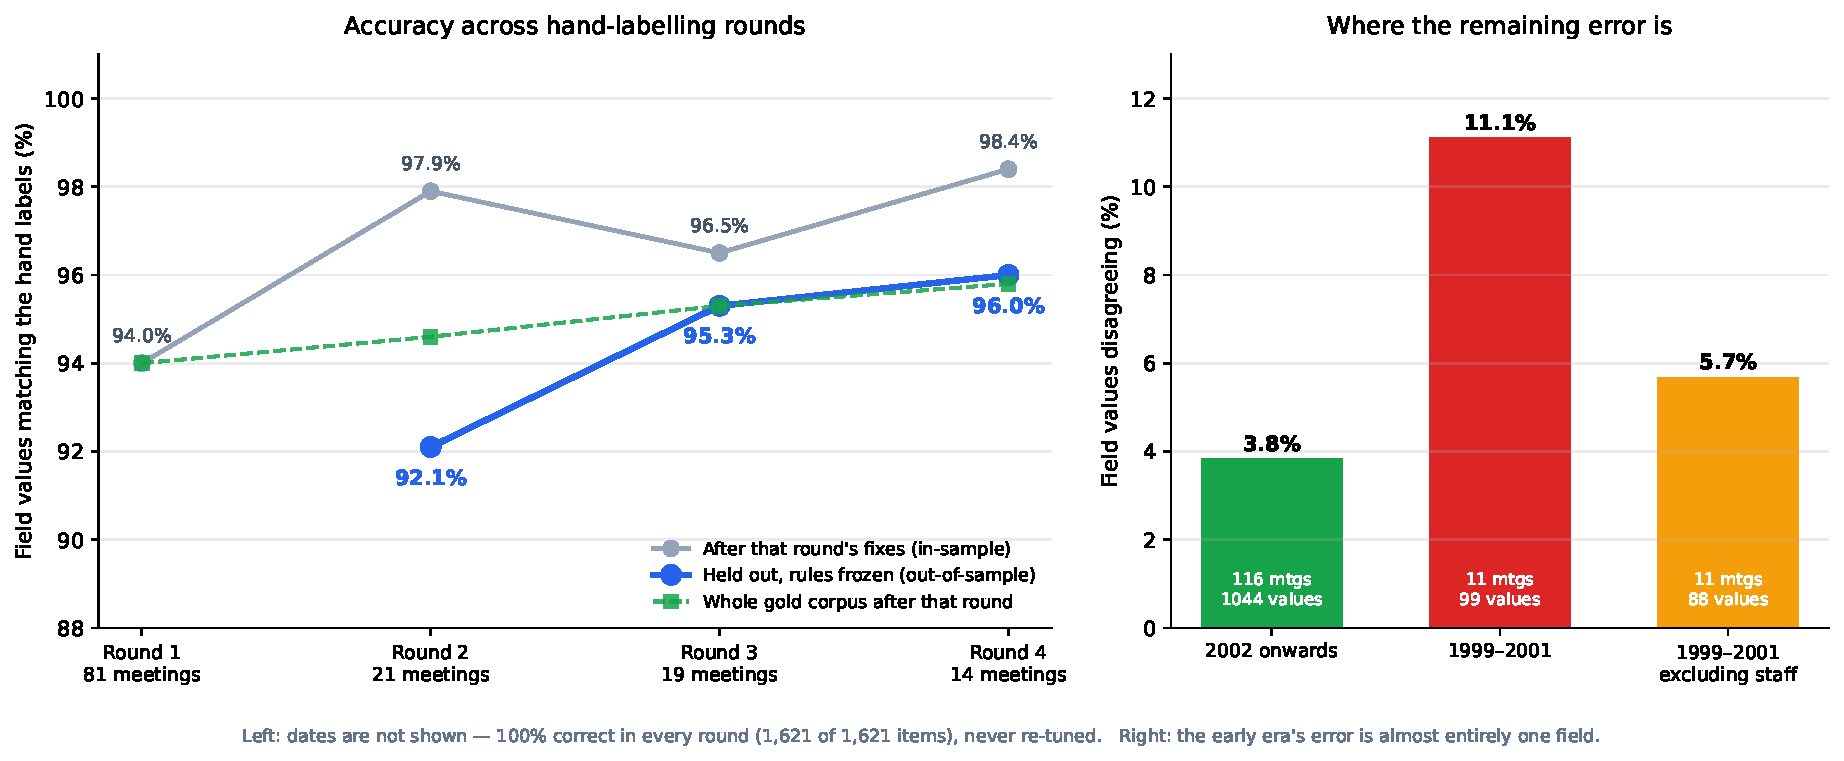
\includegraphics[width=\textwidth]{extraction_accuracy.pdf}
\caption{Left: accuracy across the four rounds. The blue line is the only generalisation
claim --- each point was measured before any rule had seen that round --- and its rise from
92.1\% to 96.0\% is the evidence that fixes transferred rather than being fitted. Right:
where the remaining error sits. The early archive costs three times the modern error rate,
and more than half of that gap is one field.}
\end{figure}

\begin{table}[h]
\centering
\resizebox{\textwidth}{!}{%
\begin{tabular}{lrrrrr}
\toprule
 & R1+R2 & \multicolumn{2}{c}{\textbf{Round 4 (14 mtgs)}} & \multicolumn{2}{c}{All (135)} \\
\cmidrule(lr){3-4}\cmidrule(lr){5-6}
Field & +R3 & \textbf{frozen} & \textbf{corrected} & 2002+ & 1999--2001 \\
\midrule
\texttt{meeting\_type}        & 100.0 & 100.0 & 100.0 & 100.0 & 100.0 \\
\texttt{meeting\_time}        & 100.0 & 100.0 & 100.0 & 100.0 & 100.0 \\
\texttt{location}             & 100.0 & 100.0 & 100.0 & 100.0 & 100.0 \\
\texttt{joint\_body}          & 100.0 & 100.0 & 100.0 & 100.0 & 100.0 \\
\texttt{joint\_body\_present} & 100.0 & 100.0 & 100.0 & 100.0 & 100.0 \\
\texttt{presiding}            &  98.3 & 100.0 & 100.0 &  98.3 & 100.0 \\
\texttt{absent}               &  95.9 &  85.7 & 100.0 &  96.6 &  81.8 \\
\texttt{present}              &  84.3 & 100.0 & 100.0 &  81.0 &  90.9 \\
\texttt{staff}                &  85.1 &  78.6 &  85.7 &  89.7 &  54.5 \\
\midrule
\textbf{All fields}           & \textbf{95.3} & \textbf{96.0} & \textbf{98.4} & \textbf{96.2} & \textbf{88.9} \\
\bottomrule
\end{tabular}}
\caption{Exact field agreement, \%. ``Frozen'' is what the rules produced on round 4 before
any correction. The last two columns split the whole gold set by era.}
\end{table}

\paragraph{The number that answers ``how accurate is this?''} \textbf{96.0\%} --- the share
of field values matching the hand labels on 14 meetings the rules had never seen, whose
\emph{boundaries the machine placed itself}. Out-of-sample accuracy has risen at every
round: 92.1\%, then 95.3\%, then 96.0\%, each measured before the rules saw the round in
question.

\paragraph{Round 4 tested something the first three could not.} Rounds 1--3 all used windows
a human had anchored by marking the meeting's header. That hid a structural gap between the
two stages.

To read a meeting's attributes, the extractor first has to decide \emph{where in the
document the meeting begins}, then cut a window of $\pm15$ lines around that point and read
the fields out of it. Everything downstream depends on that one choice of line. There are
two candidates on an archive page, and they are hundreds of lines apart:

\begin{itemize}
\item \textbf{Title-anchored} --- the page's own title and breadcrumb, at the very top:
\texttt{San Francisco Planning Department : January 11, 2001}. This is where the \emph{date}
stage anchors, and for a date it is perfectly good --- the title states it correctly, which
is why dates score 100\%. But it sits in navigation chrome: menus, font-size links, an
archived-site notice. A window cut there contains no room, no time, no roll call, because
none of those things are near it.
\item \textbf{Header-anchored} --- the meeting's own header block, roughly 230 lines further
down: \texttt{Thursday, January 11,} / \texttt{1:30 PM} / \texttt{Commission Chambers - Room
400} / \texttt{City Hall} / \texttt{PRESENT: \ldots}. Every attribute the schema asks for is
within a dozen lines of it.
\end{itemize}

\noindent
A human marking boundaries always chose the second, without being told to --- it is the
line that looks like the start of a meeting. The machine, taking the date stage's answer,
chose the first. Table~\ref{tab:anchor} is what that costs, measured over the 738 meetings
nobody has hand-labelled by counting \emph{automatic} anomalies (a field that came back
empty, a venue string that matches no known venue). Each row reads: \emph{of meetings the
machine extracted on its own, this share came back broken}. The left column is the pipeline
as it stood; the right is after adding a \texttt{snap\_to\_header} step, which walks forward
from the boundary and scores candidate lines on whether a gavel time follows closely, a roll
call follows, and a room is named just before.

\begin{table}[h]
\centering
\begin{tabular}{lrr}
\toprule
Automatic anomaly, over 738 unlabelled meetings & Title-anchored & Header-anchored \\
\midrule
No time recorded              & 84.5\% & \textbf{1.4\%} \\
No recognisable venue         & 86.0\% & \textbf{4.5\%} \\
No meeting type               & 72.9\% & \textbf{2.0\%} \\
Empty roll call               & 42.0\% & \textbf{5.7\%} \\
Empty staff list              & 24.2\% & \textbf{8.7\%} \\
\bottomrule
\end{tabular}
\caption{Share of machine-extracted meetings whose fields came back unusable, by where the
reading window was anchored. Lower is better; these are error rates, not coverage. The gold
meetings show near-zero anomalies under both anchorings, because a human had already put the
window in the right place --- which is exactly why three rounds of validation could not see
this.}
\label{tab:anchor}
\end{table}

\noindent
The practical consequence: \textbf{this is the difference between having meeting-level data
for the 135 hand-marked meetings and having it for all 1{,}179}. Round 4 then confirmed the
fix against ground truth, scoring 96.0\% with every boundary placed by machine.

\paragraph{Where the error actually is.} The gold set now spans both archive formats, and
they do not behave alike:

\begin{center}
\begin{tabular}{lrrr}
\toprule
Era & Meetings & Values & Error rate \\
\midrule
2002 onwards            & 116 & 1{,}044 & \textbf{3.8\%} \\
1999--2001              &  11 &     99 & \textbf{11.1\%} \\
1999--2001, excl.\ \texttt{staff} & 11 & 88 & \textbf{5.7\%} \\
\bottomrule
\end{tabular}
\end{center}

\noindent
The early archive costs roughly three times the modern error rate, and \textbf{more than
half of that gap is the single \texttt{staff} field}. Setting staff aside, 1999--2001 runs
at 5.7\% against 3.8\% --- a real but modest gap rather than a different regime. The cause
is one formatting habit: the 1998--2001 pages wrap header labels mid-phrase, so
\texttt{STAFF IN ATTENDANCE:} is printed as \texttt{STAFF} / \texttt{IN ATTENDANCE:} and
\texttt{THE MEETING WAS CALLED TO ORDER} as \texttt{THE} / \texttt{MEETING WAS CALLED\ldots}.
Neither half matched its pattern, so the staff roll was never found and the absence list ran
on into the gavel time and recorded ``P.M'' as a commissioner. A third bug compounded it:
the capture followed only four wrapped lines, and an early-era staff roll runs to twenty
names over six or more, so its tail --- including the Commission Secretary that ends it ---
was truncated. With all three fixed, round~4's early-era meetings score \textbf{100\%
excluding staff}.

\paragraph{The two fields that stay hard.} \texttt{present} and \texttt{staff} carry almost
all remaining error. Both are lists of six to twenty names, so one mis-parsed entry fails
the whole field under exact matching; element-wise they run near 95\% precision and recall.
For analysis that counts attendance or looks up who was there, the element figure is the
relevant one.

\paragraph{Presiding at joint meetings is a definitional rule, not an extraction problem.}
A joint session is gavelled by whichever body hosts it: on 2011-03-10 the Public Health
Commission's president called the meeting to order. But \texttt{presiding} here means
\emph{the Planning Commission's president}, because the Planning Commission is the body
whose decisions are the unit of analysis. The rule is therefore explicit: search only this
Commission's own roll-call block for a member marked President, and accept a called-to-order
name only if that person sat with the Planning Commission that day. Where neither holds the
field is left \textbf{empty} rather than filled with the other body's president --- a blank
is a question for a human, a wrong name is a silent error.

\section{Part III --- The full corpus}

The extraction described above has now been run over \textbf{every document in the corpus},
not just the hand-labelled sample: 1{,}086 documents, 1998--2026, producing
\textbf{1{,}179 meetings}. 134 of them are hand-verified; the rest carry the machine's
answer. Output is \texttt{meetings\_all.csv} and the \texttt{meetings\_all} table.

\begin{table}[h]
\centering
\begin{tabular}{lrr}
\toprule
Field & Populated & \% \\
\midrule
\texttt{location}      & 1{,}179 & 100.0 \\
\texttt{meeting\_time} & 1{,}169 &  99.2 \\
\texttt{meeting\_type} & 1{,}164 &  98.7 \\
\texttt{present}       & 1{,}137 &  96.4 \\
\texttt{staff}         & 1{,}110 &  94.1 \\
\texttt{presiding}     & 1{,}106 &  93.8 \\
\texttt{absent}        &   531 &  45.0 \\
\bottomrule
\end{tabular}
\caption{Field coverage across all 1{,}179 meetings. \texttt{absent} is low because most
meetings record no absences, not because the field fails.}
\end{table}

\paragraph{A sanity check the data passes.} \textbf{1{,}162 of 1{,}179 meetings fall on a
Thursday} (98.6\%), the Commission's sitting day. The 17 that do not are 7 Tuesdays, 5
Mondays and 5 Fridays --- special and joint sittings, which is what one would expect. No
date was ever tuned to produce this.

\subsection{Meeting type and frequency}

\begin{table}[h]
\centering
\begin{tabular}{lrrrrr}
\toprule
Period & Meetings & Regular & Special & Joint & Non-regular \\
\midrule
1998--2004 &  302 &  270 & 10 & 15 & 10.6\% \\
2005--2011 &  379 &  279 & 73 & 20 & \textbf{26.4\%} \\
2012--2018 &  222 &  194 &  4 & 15 & 12.6\% \\
2019--2026 &  276 &  261 &  1 & 14 &  5.4\% \\
\midrule
All        & 1{,}179 & 1{,}004 & 88 & 64 & 14.8\% \\
\bottomrule
\end{tabular}
\caption{Meeting type over time. 15 meetings (1.3\%) have no type recorded and 8 are closed
sessions.}
\end{table}

\noindent
The striking pattern is the \textbf{special-meeting surge in 2005--2011}: 73 of the 88
special meetings in the entire corpus fall in that seven-year window, and non-regular
sittings run at 26.4\% against 5--13\% in every other period. Whatever drove it --- the
housing cycle, a change in how the Commission scheduled contested items, or a change in how
minutes were headed --- it is a sharp and specific feature of the middle of the panel, and
it is the kind of thing the meeting level exists to surface. It deserves a look before it is
used as a covariate.

The Commission sits roughly weekly: 35--66 meetings a year, with the low years being those
where the archive itself is thin.

\subsection{Attendance}

Attendance is recorded for 1{,}137 meetings. Mean commissioners present is \textbf{6.19}
(median 6, of a seven-member Commission), and \textbf{45\% of meetings record at least one
absence}, 682 absences in total.

\begin{table}[h]
\centering
\begin{tabular}{lrrr}
\toprule
Commissioner & Absences & Meetings on roster & Rate \\
\midrule
Martin           & 29 &  71 & 40.8\% \\
Alexander        & 55 & 174 & 31.6\% \\
Chan             & 18 &  68 & 26.5\% \\
Ruiz             & 18 &  70 & 25.7\% \\
Boyd             & 17 &  79 & 21.5\% \\
Bell             & 36 & 178 & 20.2\% \\
Fay              & 13 &  74 & 17.6\% \\
Feldstein        & 11 &  71 & 15.5\% \\
Borden           & 36 & 278 & 12.9\% \\
Theoharis        & 19 & 147 & 12.9\% \\
Richards         & 19 & 149 & 12.8\% \\
\midrule
\emph{``Lee'' (unresolved)} & 36 & 192 & 18.8\% \\
\bottomrule
\end{tabular}
\caption{Absence rates for commissioners seated at 20 or more meetings. The denominator is
what makes these comparable: Borden and Alexander both show 36 and 55 raw absences, but over
very different tenures.}
\end{table}

\paragraph{One ambiguity is left visible rather than resolved.} Sue Lee and William L. Lee
both served, and many roll calls print only ``Lee''. Where the meeting says enough --- a
roll naming two Lees names both; a Lee who called the meeting to order is Sue; a bare Lee
opposite an identified Lee is the other person --- the two are separated, giving Sue Lee 232
meetings and William L. Lee 220, each with a single recorded absence. \textbf{192 meetings
retain an unresolved ``Lee''}, carrying 36 absences between them.

That row is deliberately left in the table. An earlier version assigned every unresolved
case to William, which produced a 9\% absence rate for him against 0.4\% for Sue --- an
artefact of the tie-break, not a fact about either commissioner. A visible ambiguity is
worth more than a confident wrong answer, and anyone using per-commissioner attendance
should either drop those 192 meetings or resolve them by hand.

\subsection{Who presides, where, and when}

Fong presided over 137 meetings, Olague 125, Miguel 101, Bell 88, Koppel 82, a Lee 73,
Theoharis 64, Tanner 63, Chinchilla 62 --- a genuine rotation rather than a dominant chair.

\textbf{1{,}025 meetings sat at City Hall}, 51 at the War Memorial Building (the pre-2001
home), and \textbf{80 were remote hearings} --- the pandemic-era teleconference period, now
a clean flag. Eight meetings (0.7\%) have an unrecognisable venue string.

Start times cluster hard: 480 at 1:30 PM, 294 at 12:00 PM, 212 at 1:00 PM. The shift from
1:30 to 12:00 tracks the modern era.

\textbf{64 joint sittings} are recorded, most often with the Recreation and Park Commission
(16), Building Inspection (7), Health (8 across two spellings), Historic Preservation (7
across two spellings) and the Redevelopment Agency (4).

\subsection{Two series over time}

\begin{figure}[h]
\centering

\includegraphics[width=\textwidth]{meeting_timeseries.pdf}
\caption{Staff in attendance and the commissioner absence rate, per meeting. Faint line: one
meeting. Bold line: a one-year centred moving average, windowed by \emph{calendar time}
rather than a fixed count, because the Commission's sitting frequency varies (35 meetings in
2000 against 66 in 2007). Grey bands are inferred presidency terms; purple is the
remote-hearing era.}
\label{fig:series}
\end{figure}

\paragraph{Presidency terms are inferred, not looked up.} The project holds no roster of who
chaired the Commission when, but the minutes record who called each meeting to order, and
that recovers the calendar. A raw run of the \texttt{presiding} field fragments into 188
pieces because a vice-chair takes the occasional meeting, so the series is smoothed by a
rolling mode over $\pm$7 meetings and runs shorter than six meetings are absorbed into their
neighbours. What comes out is \textbf{19 terms} averaging a little over a year each --- the
shape one would expect of an annual rotation, which is a useful check that the inference is
not manufacturing structure.

\begin{table}[h]
\centering
\small
\begin{tabular}{llrrr}
\toprule
President & Term & Meetings & Absence rate & Staff \\
\midrule
Chinchilla & 1998-01 -- 1999-01 &  47 & 15.4\% &  9.6 \\
Theoharis  & 1999-02 -- 2002-01 & 112 & 11.3\% & 10.5 \\
Bell       & 2002-05 -- 2005-01 & 106 & 10.0\% & 11.1 \\
Lee        & 2005-01 -- 2006-11 &  81 & 13.9\% & 10.7 \\
Alexander  & 2006-11 -- 2007-09 &  47 &  7.4\% &  7.8 \\
Olague     & 2007-09 -- 2009-01 &  70 &  6.6\% & 11.1 \\
Miguel     & 2009-01 -- 2011-01 &  91 &  6.2\% & 10.6 \\
Fong       & 2012-03 -- 2014-03 &  90 &  7.3\% &  9.0 \\
Wu         & 2014-03 -- 2015-02 &  35 &  2.0\% & 10.3 \\
Fong       & 2015-03 -- 2017-01 &  55 &  8.8\% &  9.4 \\
Melgar     & 2019-01 -- 2019-12 &  36 & 12.2\% & 10.4 \\
Koppel     & 2019-12 -- 2022-01 &  83 &  6.1\% &  9.7 \\
Tanner     & 2022-01 -- 2024-01 &  71 &  6.7\% &  9.4 \\
So         & 2024-09 -- 2026-03 &  56 &  7.4\% &  8.6 \\
\bottomrule
\end{tabular}
\caption{Inferred presidency terms of 35 meetings or more (five shorter terms are omitted
here but appear as bands in Figure~\ref{fig:series}). Absence rate is the mean share of the
seated Commission missing a sitting.}
\end{table}

\paragraph{The clearest pattern is not about presidents.} \textbf{Absence during remote
hearings ran at 4.9\%, against 9.1\% for in-person meetings} --- barely half. Commissioners
attended more reliably when they did not have to be in the room. Given that the panel's
whole subject is discretionary decisions made by a body that has to convene, a mechanism
that raises attendance is worth noting, though it is confounded with the period: the
2020--2022 window is also when the Commission's docket and the housing-policy environment
were unusual.

\paragraph{Absence by presidency varies more than one would expect, but tracks the era.}
The range across terms is wide --- 2.0\% under Wu against 15.4\% under Chinchilla --- yet
the pattern is chronological rather than personal: the four highest rates are the four
earliest presidencies, and Fong's two separate terms differ from each other (7.3\% then
8.8\%) by more than many presidents differ from their neighbours. That is the signature of a
period effect, not a chair effect. \textbf{We would not read these numbers as evidence that
some presidents commanded better attendance than others.} If that question matters, it needs
a specification that separates chair from period --- commissioner fixed effects and a time
trend --- rather than a comparison of term means.

\paragraph{Staff attendance shows no presidency pattern at all.} The term means sit between
7.8 and 12.6 with no relation to who is chairing, and the series drifts down slowly across
the whole panel (10.7 in 1998--2004 to 9.4 today). Two cautions: the modern PDF layout lists
staff more tersely than the HTML era did, so part of the decline may be a change in how
minutes are written; and \texttt{staff} is the least accurate field in the schema. It is
here for completeness, not as a variable to lean on.

\medskip\noindent
Both panels break at 2018, where the corpus holds only two documents. The break is drawn
rather than interpolated so a gap in the scrape is not read as a change in the Commission.

\section{Reproducing this}

\begin{verbatim}
cd code/commission_minutes_processing
python assign_meeting_dates.py --apply --sync-labels   # dates
python meeting_headers.py --export                     # meeting fields + CSV

python extract_all_meetings.py                         # ALL 1,179 meetings -> CSV + table
python plot_extraction_accuracy.py                     # the accuracy figure
python draw_validation_sample.py --seed S --round N    # a further validation round

cd date_boundary_app
python app.py                 # mark boundaries (:5006), confirm meetings (/meetings)
python app.py --score --csv   # date agreement vs the gold set
\end{verbatim}

Outputs: \texttt{date\_assignment\_audit.csv} (per page: status, headers found, items
changed), \texttt{date\_boundary\_app/date\_gold\_score.csv} (per document: gold vs detected
dates), \texttt{date\_boundary\_app/meetings\_pilot.csv} (the hand-labelled gold meetings), and
\texttt{meetings\_all.csv} (all 1{,}179 extracted meetings, with an \texttt{era} column and
a \texttt{hand\_verified} flag).

\section{Limitations}

\begin{enumerate}
\item \textbf{The ``corrected'' figures are not out-of-sample.} 96.0\% is the honest
generalisation estimate, measured on round 4 before any rule saw it. 98.4\% is what the same
meetings score after their disagreements were used to fix three defects.
\item \textbf{Dates need no such caveat.} Nothing in date assignment has changed since round
1, so 100\% item accuracy on 1{,}621 items across four rounds is a clean result.
\item \textbf{The early era is the weak spot, and it is thin.} 1999--2001 carries 11 gold
meetings and 99 field values, so its 11.1\% error rate rests on 11 disagreements. The
direction is well evidenced --- the formatting habits behind it are documented and
reproducible --- but the rate itself should be read as approximate.
\item \textbf{The gold labels are not internally consistent on names.} Five spellings for
the two Lees, and both ``Bell'' and ``Bradford-Bell'' for one person. A consistency pass
would raise measured agreement by roughly 1.5 points without changing any code.
\item \textbf{Nine documents in the corpus are landing pages, not minutes} --- a date and a
link, with no roll call or items. They should be filtered from any denominator.
\item \textbf{One boundary is marked on a page breadcrumb.} For 2010-02-18 the window covers
page chrome and no venue is recoverable. The date is unaffected.
\item \textbf{The corpus has a 2018 hole.} Only two documents exist for 2018 in
\texttt{raw/2018/}, against 27--44 for its neighbours, so 2018 is a scraping gap rather than
a year the Commission did not sit. It must be filled before any year-on-year series crosses
it.
\item \textbf{Eight meetings (0.7\%) carry an unusable venue string} and 15 (1.3\%) no
meeting type. These are visible in \texttt{meetings\_all.csv} and should be dropped or
repaired rather than analysed.
\item \textbf{The special-meeting surge of 2005--2011 is a finding, not yet an explanation.}
73 of the corpus's 88 special meetings fall in that window. It could be substantive or an
artefact of how minutes were headed in those years, and it should be checked before use.
\item \textbf{Accuracy is not uniform across the corpus.} The \texttt{era} column in
\texttt{meetings\_all.csv} exists so that downstream work can weight it: 3.8\% field error
from 2002, 11.1\% for 1999--2001.
\end{enumerate}

\appendix

\section{Appendix A --- Round 2: every held-out error, classified}

Round 2 was the first true test of the extraction machine: 21 meetings hand-labelled after
the rules were frozen, 9 fields each, 189 field values. \textbf{15 disagreed.} Every one is listed below, classified as a substantive extraction failure (the
machine read the document wrongly or not at all) or a typographic difference (the machine
and the label describe the same fact in different characters).

\begin{longtable}{p{0.12\textwidth}p{0.08\textwidth}p{0.37\textwidth}p{0.12\textwidth}p{0.12\textwidth}}
\toprule
Field & Meetings & Cause & Kind & Status \\
\midrule
\endhead
\texttt{location} & 5 & A boilerplate line (``Regular Meeting'') flushed the venue buffer,
discarding the ``City Hall'' line above it & Substantive & Fixed \\
\texttt{location} & 1 & Joint meeting: the two bodies are joined by ``\&'', so the venue
scan returned the bare separator & Substantive & Fixed \\
\texttt{staff} & 4 & The label wraps as \texttt{STAFF IN} / \texttt{ATTENDANCE:}; neither
half matched, so no staff were recorded at all & Substantive & Fixed \\
\texttt{presiding} & 1 & Joint meeting gavelled by the other body's president (Tierney,
Public Health) & Substantive (rule) & Fixed \\
\texttt{presiding} & 1 & ``\textsc{called to order by acting chair fong}'' --- only
``President'' was matched & Substantive & Fixed \\
\texttt{joint\_body} & 1 & ``\&'' rather than ``AND'' between the two commissions & Substantive & Fixed \\
\texttt{joint\_body\_present} & 1 & Same ``\&'' failure: the other body's roll call was never located & Substantive & Fixed \\
\texttt{present} & 1 & Roll-call label with its colon on the next line
(\texttt{PLANNING COMMISSIONERS PRESENT} / \texttt{:}) & Substantive & Fixed \\
\midrule
\textbf{Total} & \textbf{15} & & \textbf{15 substantive, 0 typographic} & \\
\bottomrule
\caption{The 15 held-out disagreements under frozen rules (92.1\% agreement). All were
genuine extraction failures; none was cosmetic.}
\end{longtable}

\noindent
Two things follow from this table. First, \textbf{the frozen 92.1\% is a real error rate,
not a formatting artefact} --- there is no typographic padding inflating it, so the figure
can be quoted as-is. Second, the failures cluster: eleven of the fifteen come from three
layout quirks (a wrapped staff label, a wrapped roll-call colon, an ``\&'' between two
commissions), each of which is a single pattern, and each of which is a variant the first
76 documents happened not to contain.

\subsection*{After correction}

With those six defects fixed, held-out agreement is 97.9\% --- \textbf{4 remaining errors,
and the balance inverts}:

\begin{table}[h]
\centering
\begin{tabular}{p{0.12\textwidth}rp{0.44\textwidth}p{0.18\textwidth}}
\toprule
Field & Meetings & Difference & Kind \\
\midrule
\texttt{staff} & 3 & Machine writes \texttt{John Rahaim – Director of Planning} (en dash,
as the document prints it); the label writes \texttt{-} (hyphen). Same people, same count,
same order & \textbf{Typographic} \\
\texttt{staff} & 1 & \texttt{Linda Avery – Commission Secretary. Note} --- a trailing
``. Note'' leaked past the stop marker & \textbf{Substantive} \\
\midrule
\textbf{Total} & \textbf{4} & & \textbf{1 substantive, 3 typographic} \\
\bottomrule
\end{tabular}
\caption{Residual held-out errors after correction. Normalising the dash character raises
held-out agreement from 97.9\% to \textbf{99.5\%} (188/189), leaving a single genuine
extraction error across 21 meetings.}
\end{table}

\noindent
The dash is preserved rather than standardised on purpose: the corpus mixes \texttt{-} and
\texttt{–}, and an earlier version that rewrote one as the other was reverted, because
silently altering characters is the kind of change that looks harmless and then bites at
join time. If a single canonical dash is wanted downstream, the right place for it is a
normalisation at export, leaving the stored value faithful to the source.


\section{Appendix B --- Round 3: every held-out error, classified}

Round 3 was a seeded random draw of 20 documents from the 989 not yet marked --- 19 real
meetings plus one landing page correctly left unlabelled. 171 field values, \textbf{8
disagreed} (95.3\%).

\begin{table}[h]
\centering
\begin{tabular}{p{0.11\textwidth}rp{0.46\textwidth}p{0.16\textwidth}}
\toprule
Field & Mtgs & Cause & Kind \\
\midrule
\texttt{staff} & 4 & The roll ran past the Commission Secretary into
``\textsc{consideration of items proposed for continuance}\ldots'' & Substantive \\
\texttt{present} & 2 & A section-letter stop fired on the initial in ``S. Lee'',
emptying the roll call & Substantive \\
\texttt{staff} & 1 & A doubled dash from spacing normalisation
(``Boyajian - - Deputy City Attorney'') & Typographic \\
\texttt{presiding} & 1 & An all-capitals name on a joint meeting returned uncased
(``BELL'') & Typographic \\
\midrule
\textbf{Total} & \textbf{8} & & \textbf{6 substantive, 2 typographic} \\
\bottomrule
\end{tabular}
\caption{The 8 round-3 disagreements under frozen rules. Compare Appendix A: round 2 had 15
errors on a similar number of values, and all were substantive.}
\end{table}

\noindent
Two things are worth reading off this comparison. The error count nearly halved between
rounds (15 $\to$ 8) on documents drawn at random rather than from a chosen month, which is
the same signal the blue line in Figure 1 carries. And the failures again \textbf{cluster
into a few named causes} rather than scattering: four of eight are one endpoint --- where
the staff roll stops --- exactly as eleven of fifteen in round 2 came from three layout
quirks. That is the shape of the remaining risk: not gradual imprecision, but occasional
unseen layout variants that fail loudly and are cheap to fix once seen.

\subsection*{After correction}

With those defects fixed, round 3 stands at 96.5\% --- \textbf{6 residual disagreements, none
of them an extraction error}:

\begin{table}[h]
\centering
\begin{tabular}{p{0.11\textwidth}rp{0.46\textwidth}p{0.16\textwidth}}
\toprule
Field & Mtgs & Difference & Kind \\
\midrule
\texttt{present}, \texttt{absent} & 3 & Machine writes ``Bell''; the label writes
``Bradford-Bell''. One person, two spellings & Label convention \\
\texttt{present} & 2 & Machine writes ``William L. Lee'' by the president rule; the label
writes a bare ``Lee'' & Label convention \\
\texttt{staff} & 1 & The label ran two rolls into one entry (``\ldots Commission Secretary
\emph{Redevelopment Staff In Attendance: Erwin R. Tanjuaquio}'') & Label error \\
\midrule
\textbf{Total} & \textbf{6} & & \textbf{0 extraction errors} \\
\bottomrule
\end{tabular}
\caption{Residual round-3 disagreements. In every case the machine follows a stated rule and
the hand label does not, which is why the gold set is due a consistency pass.}
\end{table}


\section{Appendix C --- Round 4: machine-placed boundaries, every error classified}

Round 4 differed from its predecessors in two ways. The ten documents were drawn
\emph{weighted by measured anomaly rate} rather than uniformly --- allocating slots by year
first, because 1999 is the most anomalous year at 45\% but holds only eleven unmarked
documents, so weighting documents directly lets a large clean year outvote it. And the
boundaries were placed by the machine, not by hand. The draw averaged a 20.9\% anomaly rate
against 15.1\% for a uniform draw, and yielded 14 meetings because two of the ten documents
are monthly compilations.

171 field values were compared; \textbf{5 disagreed} (96.0\%).

\begin{table}[h]
\centering
\begin{tabular}{p{0.10\textwidth}rp{0.48\textwidth}p{0.16\textwidth}}
\toprule
Field & Mtgs & Cause & Kind \\
\midrule
\texttt{staff} & 2 & The label is printed \texttt{STAFF} / \texttt{IN ATTENDANCE:} across two
lines in 2000; neither half matched, so no staff were recorded & Substantive \\
\texttt{absent} & 2 & \texttt{THE} / \texttt{MEETING WAS CALLED TO ORDER\ldots} also wraps, so
the absence list ran on and recorded ``P.M'' as a commissioner & Substantive \\
\texttt{staff} & 1 & The capture followed only four wrapped lines; a 1998 staff roll runs to
twenty names over six, so its tail --- including the Commission Secretary --- was truncated
& Substantive \\
\midrule
\textbf{Total} & \textbf{5} & & \textbf{5 substantive} \\
\bottomrule
\end{tabular}
\caption{The 5 round-4 disagreements under frozen rules. All five are the same underlying
phenomenon: the early archive wraps header labels mid-phrase, and the captures were not
built for it.}
\end{table}

\noindent
Every error fell in 1998--2001; the seven meetings from 2002 onward scored \textbf{100\%}.
With the three fixes applied, round 4 stands at 98.4\%, and its early-era meetings score
\textbf{100\% excluding staff}.

\paragraph{What round 4 establishes.} Machine-placed boundaries work. The whole round ran
without a human marking a single meeting start, and the fields still agreed with the hand
labels on 96\% of values before correction --- which is the evidence that meeting-level data
can be produced for all 818 meetings rather than only the 135 that have been hand-marked.
The residual risk is now well localised: one archive format, one field, one formatting
habit.

\end{document}
